\chapter{序論}
欧州原子力研究機構(\textbf{CERN})に設置されている大型ハドロン衝突型加速器(\textbf{LHC})では、現在、素粒子物理学の基礎となっている標準模型の精密測定や標準模型を超える物理現象の探索が行われている。
ATLAS実験はLHC上にある4つの衝突点の1つで行われている実験であり、ATLAS検出器を用いて崩壊粒子の測定が行われている。LHCでは加速器のアップグレード(\textbf{HL-LHC})を予定しており、これに向けてATLAS検出器のアップグレードを行う。この章ではLHC-ATLAS実験とそのアップグレード計画について説明する。

\section{素粒子物理と標準模型}
hoge

\section{LHCについて}
LHCはCERNの地下およそ100 $\rm{m}$に設置されている周長26.7 $\rm{km}$の大型ハドロン衝突型加速器である。
バンチと呼ばれる陽子のかたまりを7 $\rm{TeV}$まで加速し、衝突させる。世界最大エネルギーの加速器である。

陽子ビームの加速は4つの前段加速器を用いて行う。始めに水素ガス中の水素原子から電子を分離することで陽子を生成する。
その後最初の線形加速器(Linear Accelarator: LINAC)、陽子シンクロトロンブースター(Proton Synchrotron Booster: PSB)、陽子シンクロトロン(Proton Synchrotron: PS)、スーパー陽子シンクロトロン(Super Proton Synchrotron)で加速されたのちLHCに入射する。CERNにある加速器の概要を図\ref{LHC_overview}に示す。
LHCには4つの衝突点があり、それぞれALICE(A Large Ion Collider Experiment)、LHCb、CMS(Compact Muon Solenoid)、ATLAS(A
Troidal LHC Apparatus)実験が行われている。それぞれの衝突点には崩壊粒子の飛跡やエネルギーを測定するための検出器が設置されており、取得したデータを元に多様な物理解析が行われている。

\begin{figure}[bpt]\centering
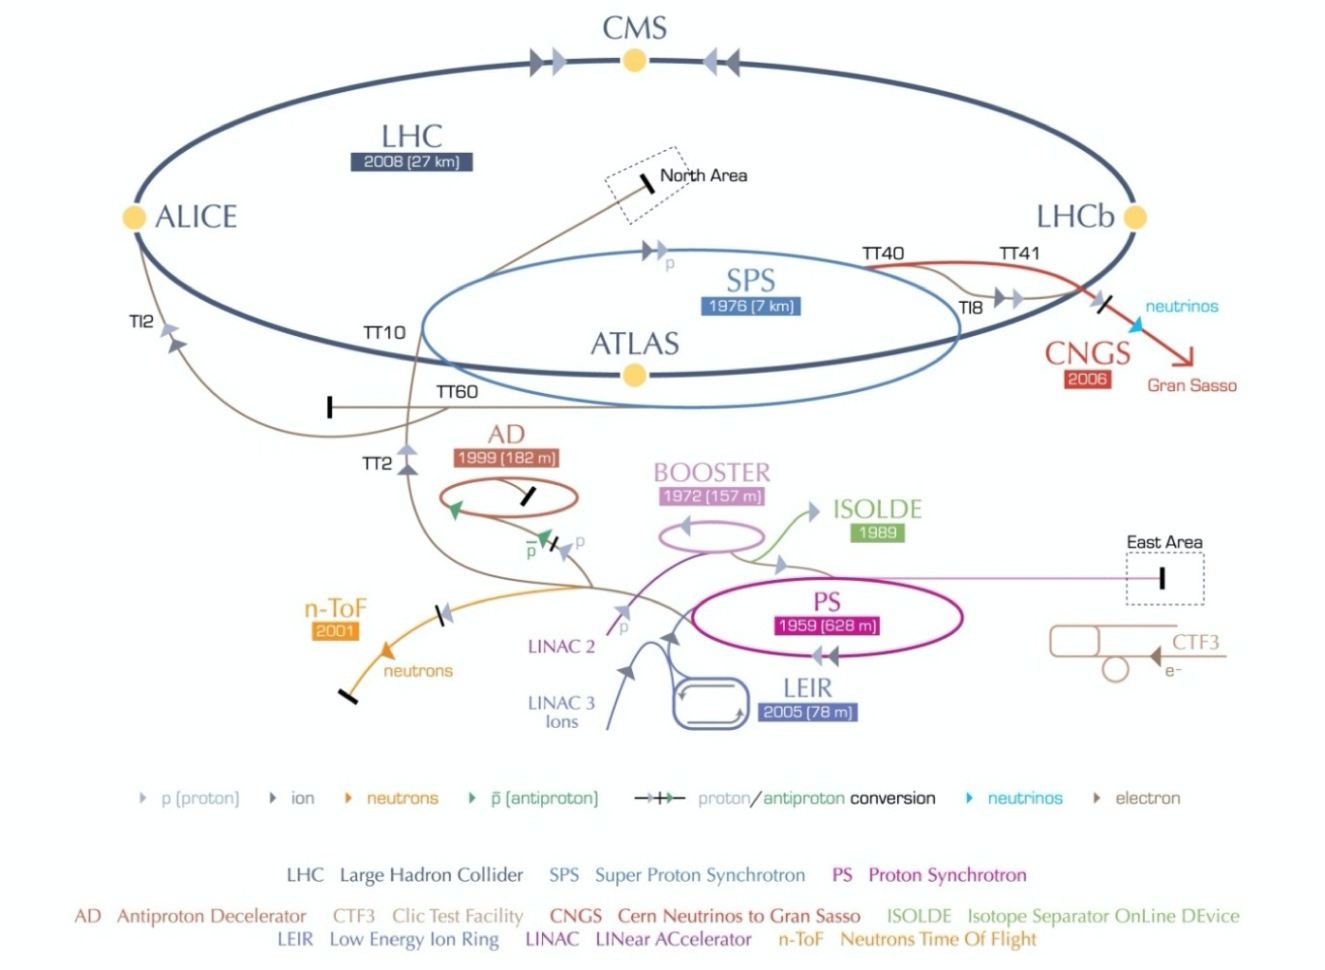
\includegraphics[width=12cm]{./LHC_overview.png}
\caption[加速器の全体像]{加速器の全体像\cite{1-1}。図はCERNに設置されている加速器の全体像を示す。陽子はいくつかの前段加速器で段階的に加速されLHCに入射する。LHC上には4つの衝突点が存在し、それぞれALICE、LHCb、CMS、ATLAS実験が行われている。}
\label{LHC_overview}
\end{figure}

\section{ATLAS実験}
初めにATLAS実験に用いる座標系と用語について説明する。まず衝突点を原点として定義しており、ビーム軸を$z$軸、これに対して垂直な平面を$x-y$平面とする。
$x$軸方向は原点からみてLHCリングの中心に向かう方向であり、$y$軸は上に向かう方向である。
方位角$\phi$は$z$軸周りの角度であり、極角$\theta$は$z$軸とのなす角である。ATLAS実験では、極角$\theta$は以下のように擬ラピディティ$\eta$で表される。
また極角$\theta$と擬ラピディティ$\eta$の関係図を図\ref{eta_theta_graph}に示す。
\bbb
\eta = -\rm{ln \left( tan\left(\frac{\theta}{2}\right) \right) }
\label{eta_theta}
\eee

\begin{figure}[bpt]\centering
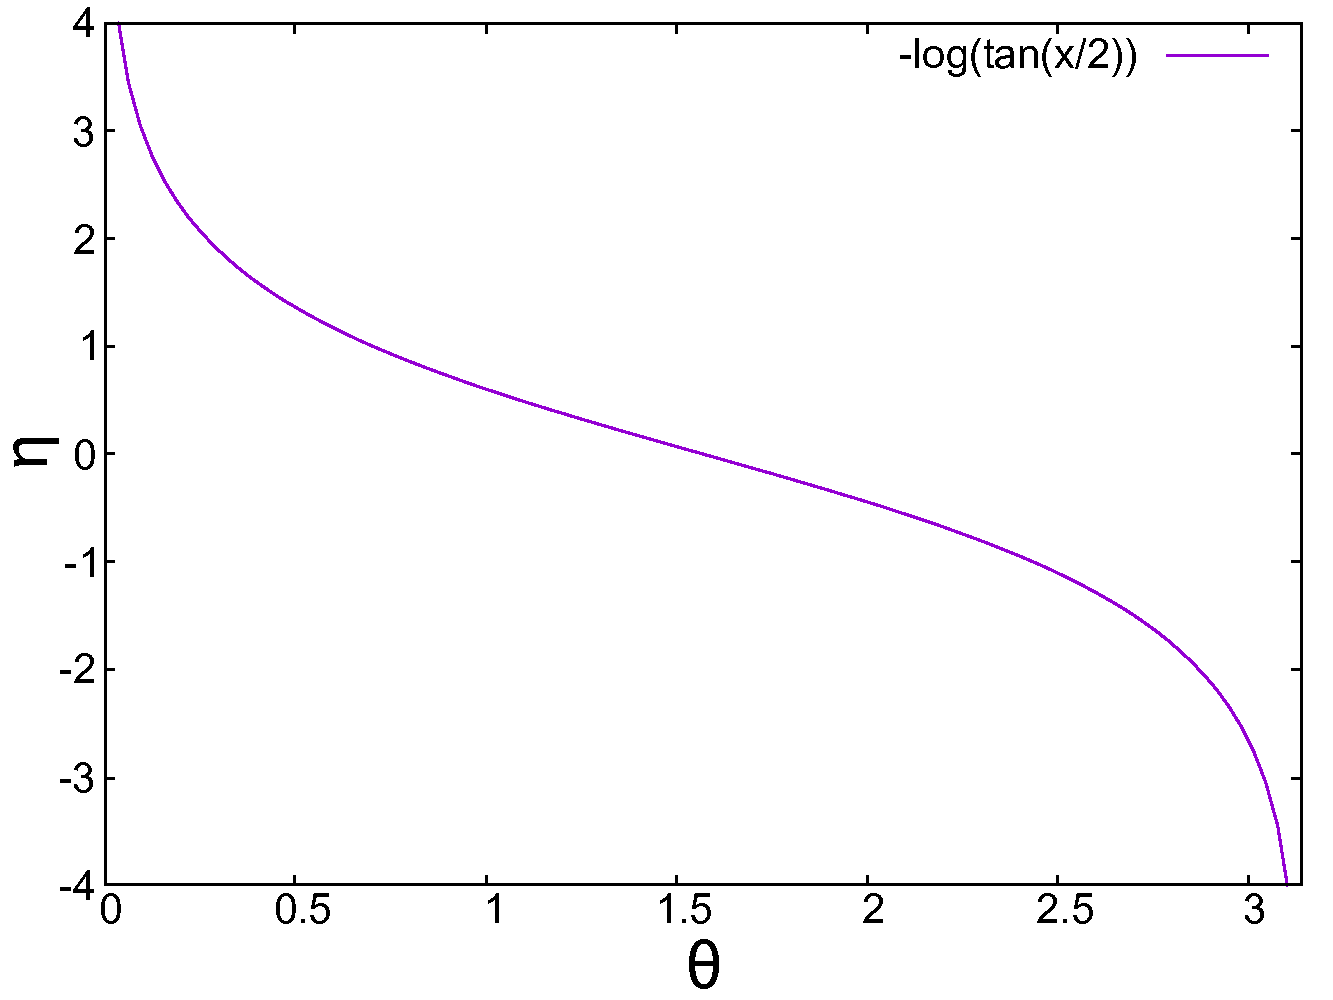
\includegraphics[width=6cm]{./data/eta_theta_relation.pdf}
\caption[極角$\theta$と擬ラピディティ$\eta$の関係図]{極角$\theta$と擬ラピディティ$\eta$の関係図。横軸は式\ref{eta_theta}における極角$\theta (0\leq\theta\leq\pi)$、縦軸は擬ラピディティ$\eta$を表している。図のように、$\eta$への変換により定義域が実数全体に広がる。}
\label{eta_theta_graph}
\end{figure}

\subsection{ATLAS検出器}
ATLAS検出器は複数の検出器から構成され、陽子の衝突によって生成された粒子の運動量、エネルギーを測定することができる。
最内層に内部飛跡検出器が設置されていて、次に超電導ソレノイド磁石、カロリメータ、トロイド磁石、ミューオン検出器の順に設置されている。ビームパイプ以外をほとんど検出器で覆うような設計となっている。
ATLAS検出器の全体図を図\ref{atlas_detector}に示す。

\begin{figure}[bpt]\centering
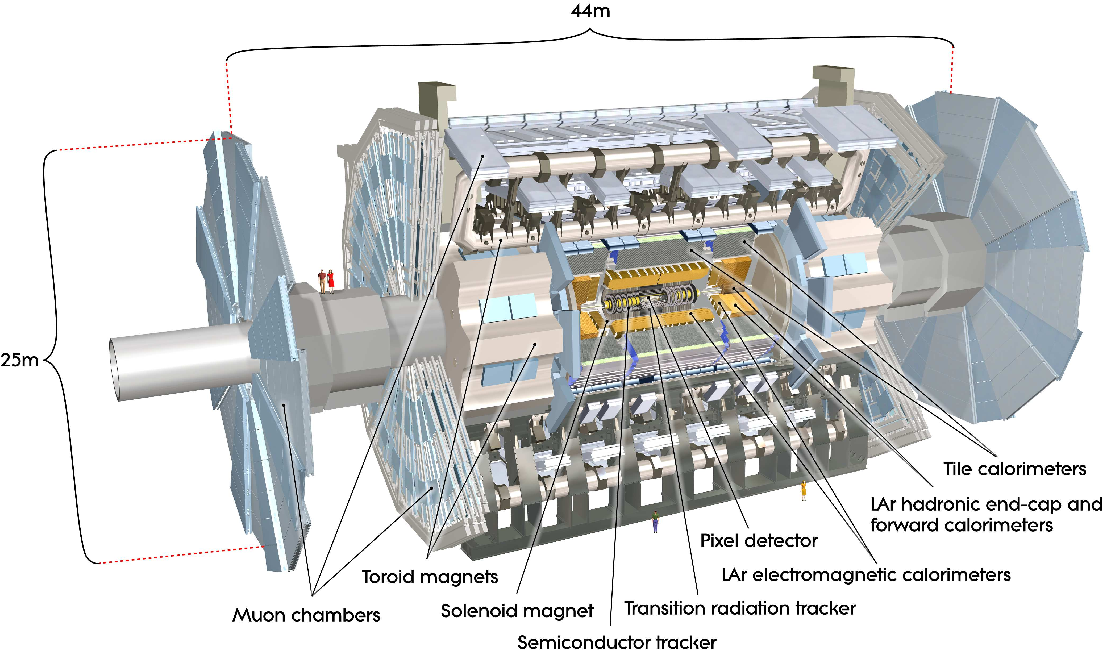
\includegraphics[width=10cm]{./atlas_detector.png}
\caption[ATLAS検出器の全体像]{ATLAS検出器の全体像\cite{1-2}。内側から内部飛跡検出器、ソレノイド磁石、カロリメータ、トロイド磁石、ミューオン検出器が設置されている。}
\label{atlas_detector}
\end{figure}

%\begin{figure}[bpt]\centering
%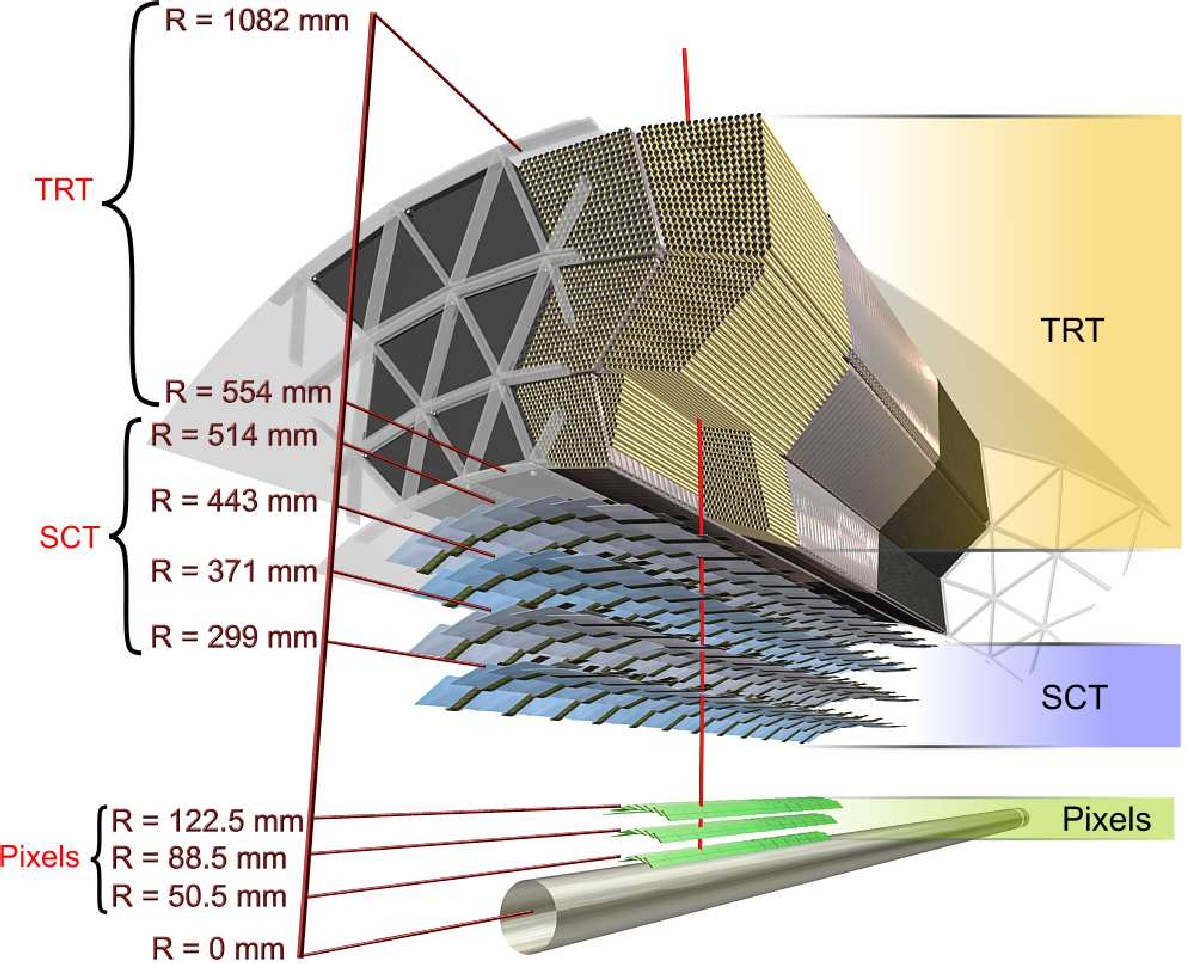
\includegraphics[width=10cm]{atlas_detector_cross_section}
%\caption[ATLAS検出器]{ATLAS検出器\cite{1-2}}
%\label{atlas_detector_cross_section}
%\end{figure}

\subsection{内部飛跡検出器}
ATLAS検出器の最内層に位置する検出器である。
内部飛跡検出器は粒子の飛跡測定をするための検出器であり、飛跡の曲率から粒子の運動量を計算できる。
検出器の外側には超伝導ソレノイド磁石が設置されており、2 $\rm{T}$の磁場が$z$方向にかけられる。これにより荷電粒子はローレンツ力を受け、軌跡が曲がる。

内部飛跡検出器は3つの検出器で構成され、内側からピクセル検出器、ストリップ検出器、遷移放射検出器の順に設置されている。
ピクセル、ストリップ検出器は階層構造になっており、粒子は複数の検出器を通過する。
それぞれの検出器で取得した通過位置をつなぎ合わせることで粒子の軌跡を計算することができる。

内部飛跡検出器の全体図を図\ref{inner_detector}に示す。

\begin{figure}[bpt]\centering
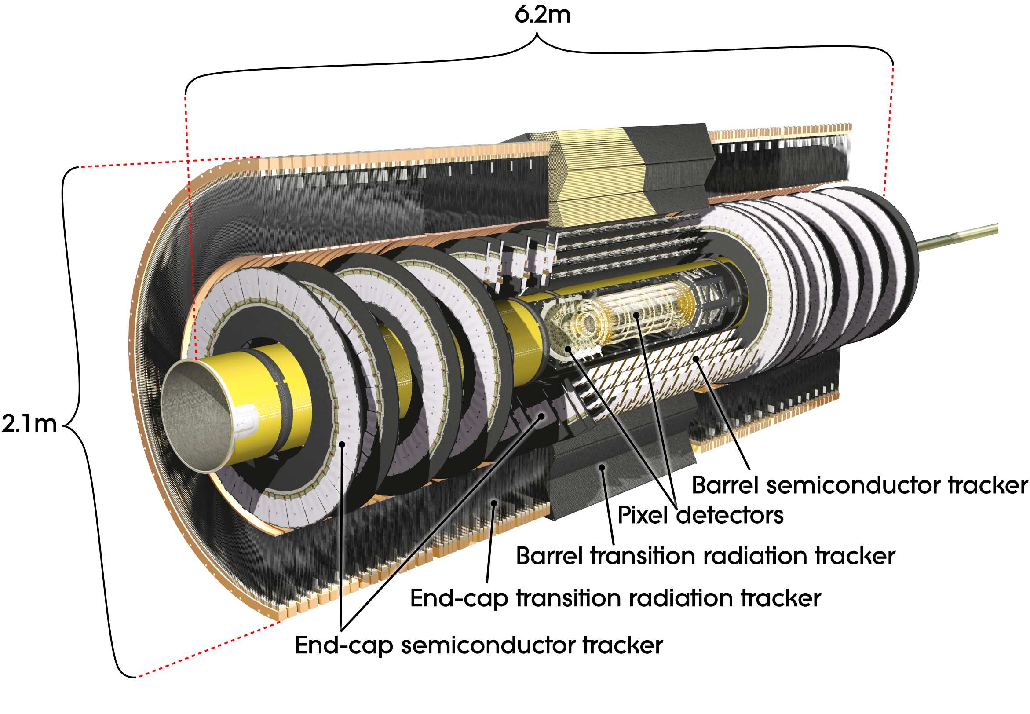
\includegraphics[width=10cm]{./inner_detector.png}
\caption[内部飛跡検出器の全体像]{内部飛跡検出器の全体像\cite{1-2}。内側からピクセル検出器、ストリップ検出器、遷移放射検出器が設置されている。また円筒状のバレル部とディスク上のエンドキャップ部を構造として持つ。}
\label{inner_detector}
\end{figure}


%検出器は$\eta$の範囲によってバレル部とエンドキャップ部に分かれる。図\ref{inner_cross_section}にビーム軸方向の端面図を示す。
%
%\begin{figure}[bpt]\centering
%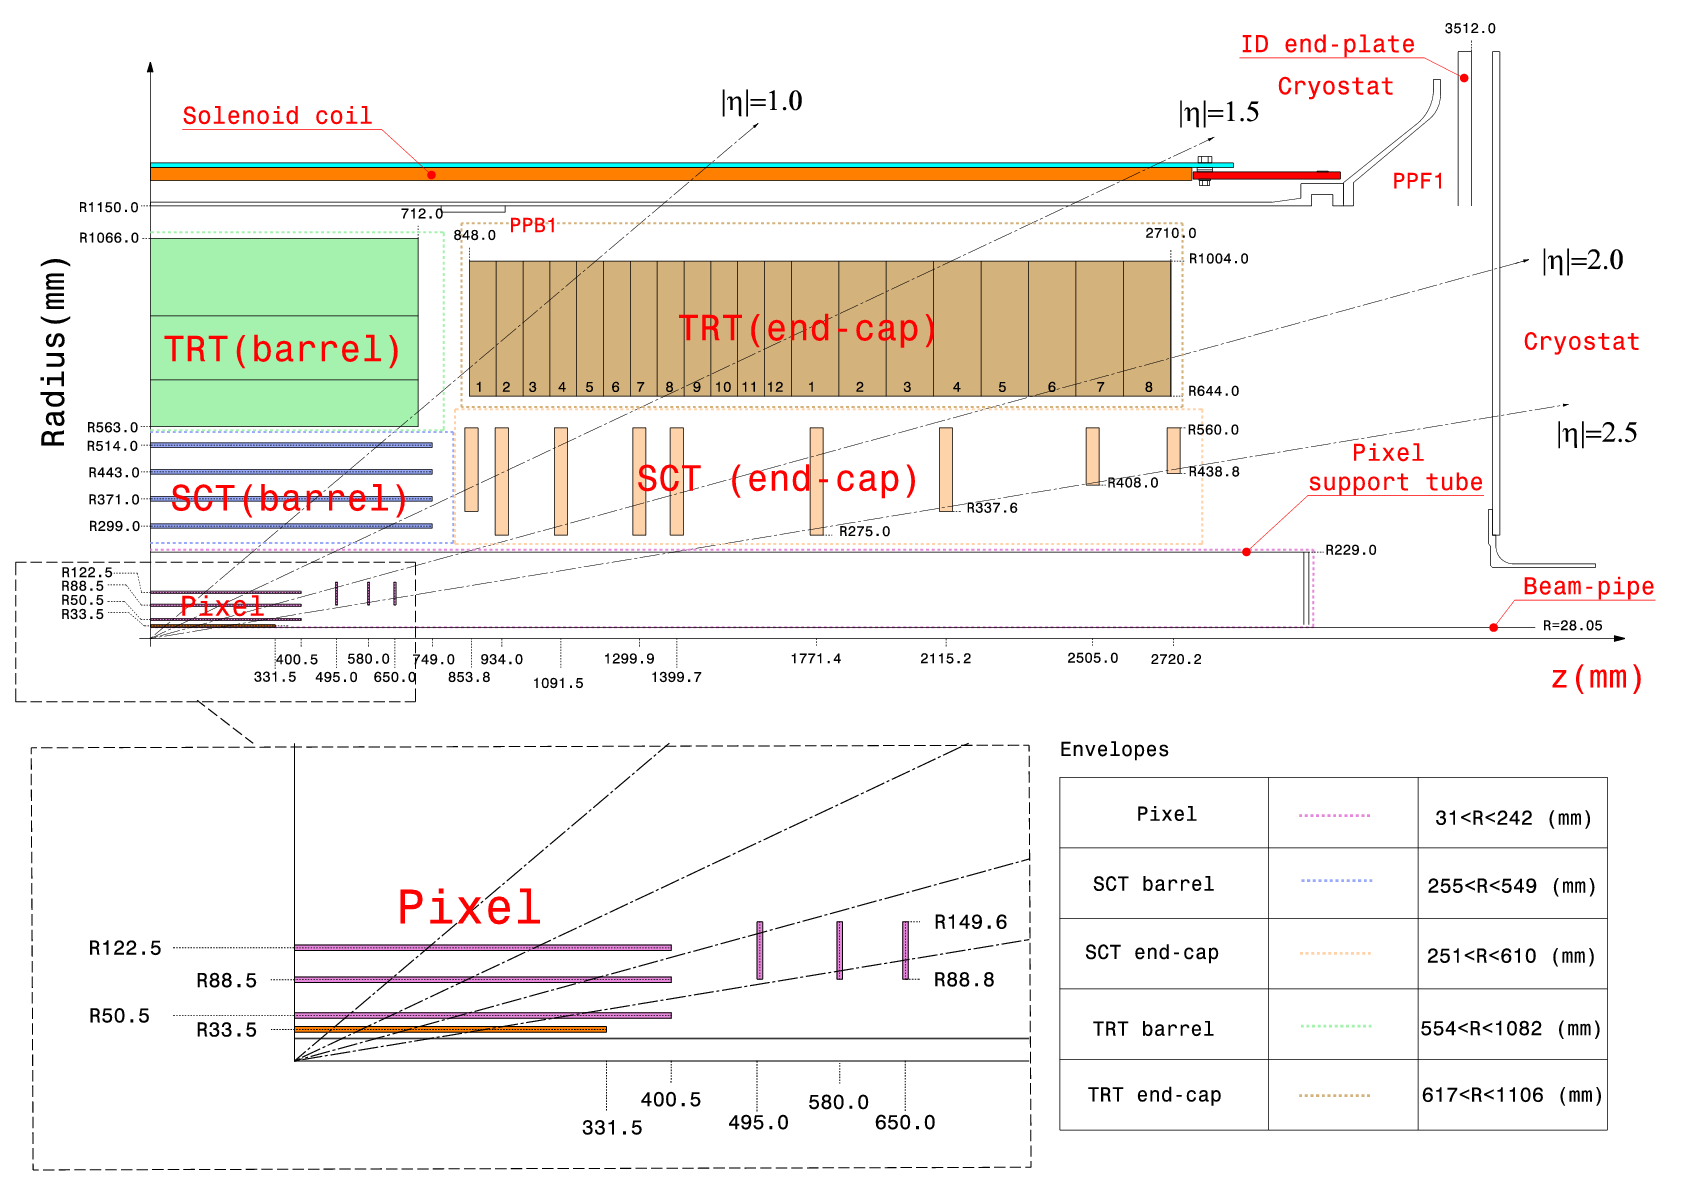
\includegraphics[width=12cm]{./inner_cross_section.png}
%\caption[内部飛跡検出器]{内部飛跡検出器\cite{1-4}}
%\label{inner_cross_section}
%\end{figure}

\subsubsection{ピクセル検出器}

内部飛跡検出器の最内層に位置する検出器である。
ピクセル検出器はバレル部が4層、エンドキャップ部が6層で構成される。
バレル部の最内層はIBL(Insertable B-Layer)と呼ばれ、順にB-Layer、Layer-1、Layer-2となっている。

ピクセル検出器の全体図を図\ref{pixel_detector_overview}に示す。
\begin{figure}[bpt]\centering
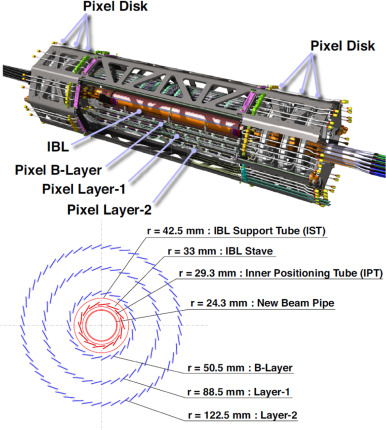
\includegraphics[width=8cm]{./pixel_detector_overview.jpg}
\caption[ピクセル検出器の全体像]{ピクセル検出器の全体像\cite{1-5}。上図はピクセル検出器の全体を模式的に表したものであり、下図はビーム軸方向から見たピクセル検出器の断面図である。バレル部の4層は内側からIBL、B-Layer、Layer-1、Layer-2と呼ぶ。}
\label{pixel_detector_overview}
\end{figure}

ピクセル検出器の各層は、モジュールと呼ばれる最小単位の検出器をいくつも搭載している。
ピクセルモジュールを図\ref{pixel_detector}に示す。
このピクセルモジュールの詳細については2章で述べる。
\begin{figure}[bpt]\centering
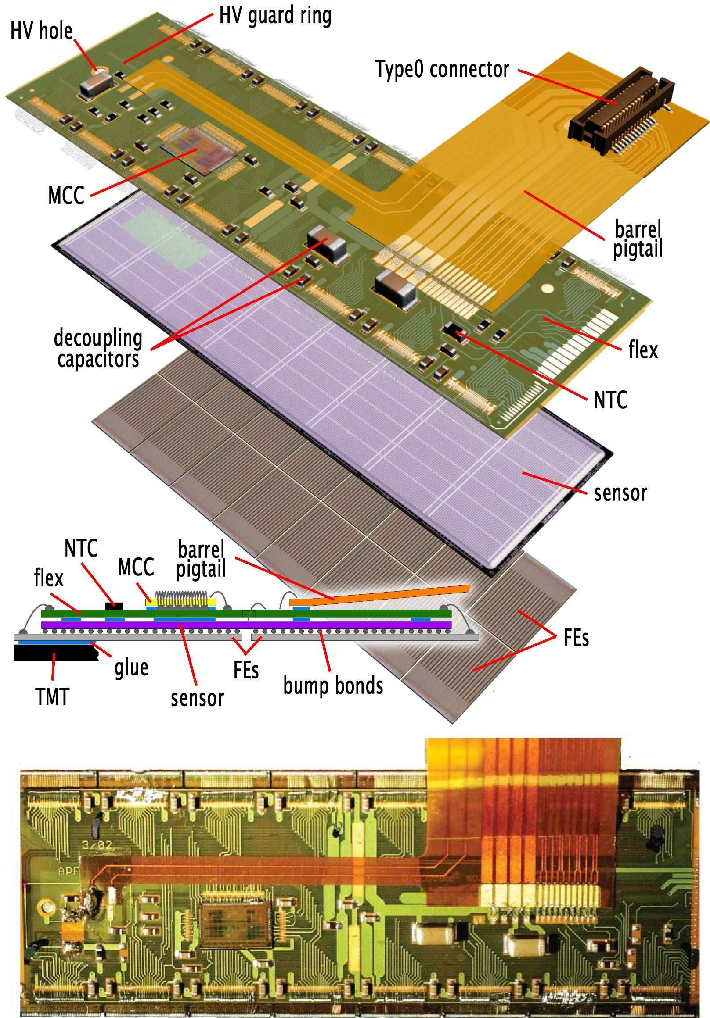
\includegraphics[width=6cm]{./pixel_detector.png}
\caption[ピクセルモジュールの全体像。]{ピクセルモジュールの全体像\cite{1-2}。ピクセル検出器は、最小単位としてモジュールと呼ばれる構造を持ち、図にモジュールの全体像を示している。モジュールは、荷電粒子が通過し、信号を生成するセンサー部、AD変換を行うFEチップ部、データ転送を行うフレキシブル基板から構成される。}
\label{pixel_detector}
\end{figure}


\clearpage
\section{HL-LHC実験アップグレード計画}
LHCでは加速器のアップグレードを予定しており、これをHL-LHCアップグレード計画と呼ぶ。詳細を以下に示す。
\subsection{概要}
HL-LHCではルミノシティ呼ばれる陽子バンチの密度を上げることで、衝突頻度を大きくし、取得統計数を増やす目的がある。
LHCとHL$-$LHCの比較を表\ref{compare_lhc}に示す。

\begin{table}[tbp]
\begin{center}
\caption[現行LHCとHL-LHCの比較]{現行LHCとHL-LHCの比較\cite{1-6}。瞬間ルミノシティは7倍、積分ルミノシティは10倍になることが見積もられており、取得統計数の増加が期待できる。}
\label{compare_lhc}
  \begin{tabular}{|lll|} \hline
    & LHC & HL$-$LHC \\ \hline
    重心系エネルギー & 14 & 14 \\
    瞬間ルミノシティ[$\rm{cm^{-2}s^{-1}}$] & $1\times 10^{34}$ & $7\times10^{34}$ \\
    積分ルミノシティ[$\rm{fb^{-1}}$] & $300$ & $3,000$ \\
    1陽子衝突あたりのイベント数 & $27$ & $140$ \\ \hline 
  \end{tabular}
\end{center}
\end{table}

LHCの運転計画を表\ref{hllhc_plan}に示す。
2025年の初めよりHL-LHCの導入が始まり、2027年の途中からHL-LHC運転開始の予定となっている。
\begin{figure}[bpt]\centering
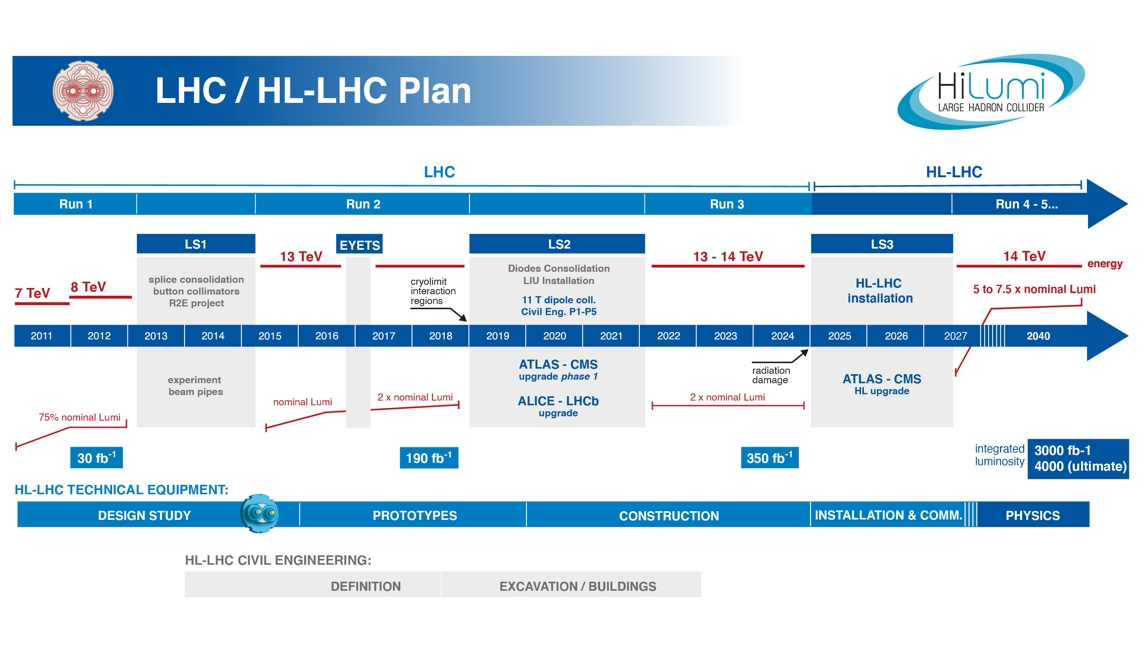
\includegraphics[width=12cm]{./hllhc_plan.jpg}
\caption[HL-LHC運転計画]{HL-LHC運転計画\cite{1-7}。2025年の初めよりHL-LHCの導入、2027年の途中より本運転が始まる。}
\label{hllhc_plan}
\end{figure}

\subsection{内部飛跡検出器のアップグレード}
ルミノシティの増加に伴い、検出器には以下のような性能が要求される。
\begin{itemize}
  \item 放射線耐性の向上.\\
  統計量に伴い、放射線量も増加するため高放射線耐性が要求される。
  \item 高速読み出し.\\
  ルミノシティの増加にするため、現行よりも高速な読み出しが要求される。
  \item 検出器の細密化.\\
  1バンチ衝突あたりのイベント数が表\ref{compare_lhc}より約5倍になる。これらの衝突点を区別するためにはより細密な検出器で位置測定を区別する必要がある。図\ref{detector_posi_res}にイメージを示す。
\end{itemize}

\begin{figure}[bpt]\centering
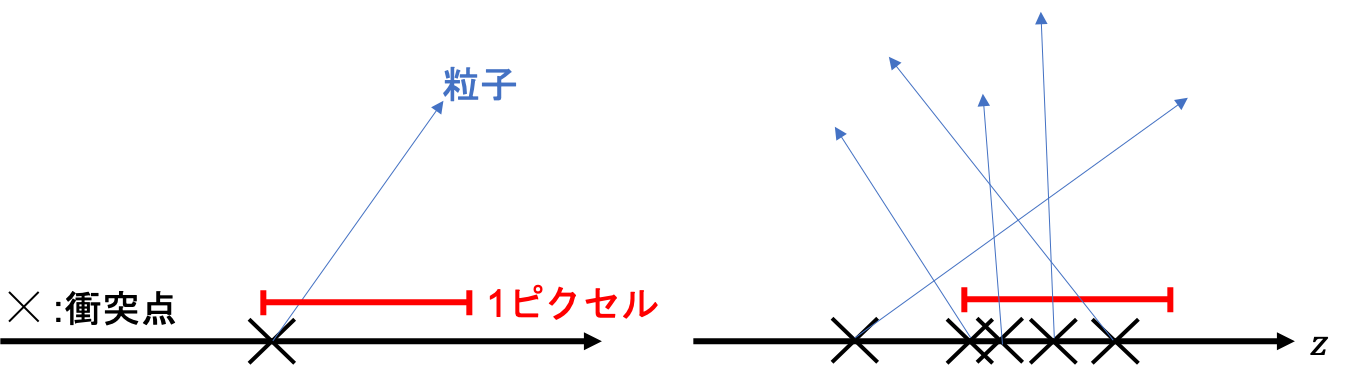
\includegraphics[width=12cm]{./detector_posi_res.png}
\caption[1バンチ衝突あたりのイベント数増加のイメージ]{1バンチ衝突あたりのイベント数増加のイメージ。図において黒先がビーム軸と衝突点、青線が生成粒子、赤線が1ピクセルを表す。左図がLHC、右図がHL-LHCの様子を表している。HL-LHCでは1バンチ衝突あたりのイベント数が約5倍に増えるため、図のように衝突点の間隔が小さくなる。これらを区別するためには今までよりも細密な検出器を設置する必要がある。}
\label{detector_posi_res}
\end{figure}

HL-LHCに向けて内部飛跡検出器はアップグレードを予定しており、検出器の総入れ替えを行う。
アップグレード後の検出器を\textbf{Inner Tracker(ITk)}と呼ぶ。模式図を図\ref{itk_image}に示す。

\begin{figure}[bpt]\centering
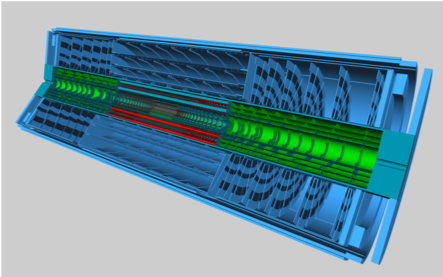
\includegraphics[width=10cm]{./itk_image.png}
\caption[ITkの全体像]{ITkの全体像\cite{1-3}。図はITk全体の模式図を示している。ITkはピクセル検出器(緑の領域)とストリップ検出器(青の領域)から構成される。}
\label{itk_image}
\end{figure}

\subsubsection{ITkの構成と現行ピクセル検出器との比較}
図\ref{itk_cross_section}にITkのビーム軸方向の断面図を示す。
ITkはピクセル検出器とストリップ検出器で構成される。
ピクセル検出器はバレル、傾斜バレル、エンドキャップ部で構成され、バレル部は5層となっている。

\begin{figure}[bpt]\centering
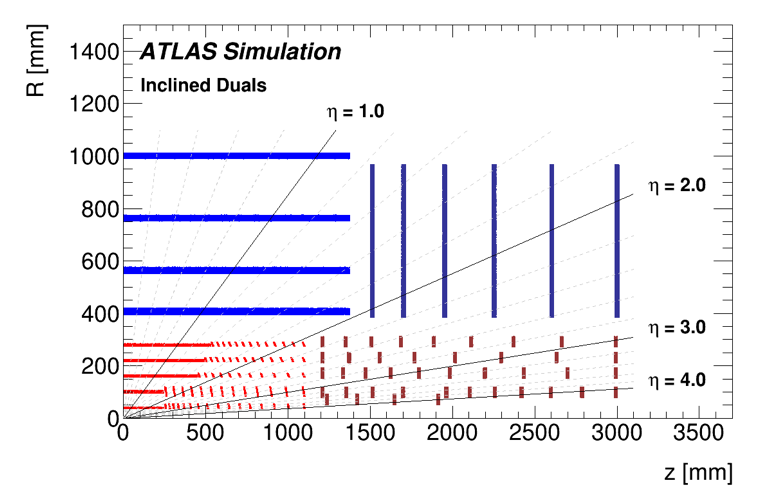
\includegraphics[width=12cm]{./itk_cross_section.png}
%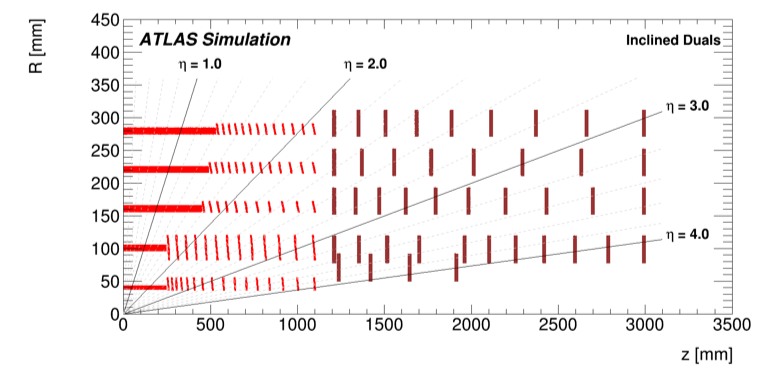
\includegraphics[width=10cm]{itk_pixel_cross_section}
\caption[ITkの断面図]{ITkの断面図\cite{1-3}。ITkはピクセル検出器とストリップ検出器から構成され、バレル部はそれぞれ5、4層の構造を持つ。ピクセル検出器はバレル部、傾斜バレル部、エンドキャップ部に分かれ、$|\eta|<4.0$までの範囲をカバーし、粒子の飛跡測定をすることができる設計となっている。}
\label{itk_cross_section}
\end{figure}

ピクセル検出器の配置に関して、現行とITkの比較を表\ref{compare_itk_pixel}に示す。
またモジュール数の比較を表\ref{compare_itk_modules}に示す。
ITkでは現行に比べ、$\eta$が大きい領域まで検出器を設置するため、その分使用するモジュール数も増える。

\begin{table}[tbp]
\begin{center}
\caption[ピクセル検出器設置領域の比較]{ピクセル検出器設置領域の比較。表は現行とITkにおけるピクセル検出器設置領域の比較を示す。$\eta$の範囲に関して、括弧内は度数法における対応する値を示す。ITkでは遷移放射検出器を使用しないため、ピクセル検出器の半径方向のカバー領域が増え、層の数は4から5となる。また前方方向に生じる粒子測定を行うために、$\eta$の領域も拡大している。}
\label{compare_itk_pixel}
  \begin{tabular}{|lll|} \hline
    & 現行 & ITk \\ \hline
    $r[\rm{mm}]$ & $33〜129$ & $39〜279$ \\ 
    層の数(バレル部) & 4 & 5 \\ 
    $|\eta|$ & $<2.5~(<19^\circ)$ & $<4~(<4.2^\circ)$ \\ \hline
  \end{tabular}
\end{center}
\end{table}

\begin{table}[tbp]
\begin{center}
\caption[搭載するピクセルモジュール数の比較]{搭載するピクセルモジュール数の比較。表は現行とITkのピクセル検出器において、各構造における搭載ピクセルモジュールの数を示している。ITkではバレル部で現行の約2倍になっているのに加え、傾斜バレル部、エンドキャップ部に多くのモジュールを搭載する設計となっていることが分かる。}
\label{compare_itk_modules}
  \begin{tabular}{|l||ll|ll|ll|} \hline
          & バレル部 &            & 傾斜バレル部 & & エンドキャップ部 & \\ \hline 
    層    & 現行     & ITk        & 現行& ITk          & 現行  & ITk \\ \hline
    1     & $280$    & $192$      & $-$ & $512$        & $-$   & $64$ \\ 
    2     & $286$    & $240$      & $-$ & $520$        & $-$   & $242$ \\ 
    3     & $494$    & $660$      & $-$ & $660$        & $-$   & $320$ \\ 
    4     & $676$    & $960$      & $-$ & $1040$       & $288$ & $352$ \\ 
    5     & $-$      & $1300$     & $-$ & $1300$       & $-$   & $468$ \\ \hline
    合計  & $1736$   & $3352$     & $0$ & $4032$       & $288$ & $1446$ \\ \hline\hline
  \end{tabular}
\end{center}
\end{table}

\subsection{物理測定に及ぼす影響}
カバーする$\eta$の範囲が大きい特徴が生む利点として、前方方向に大きな運動量を持つ粒子を含む物理現象の測定精度向上があげられる。

この例として、ボゾン粒子結合によるヒッグス粒子生成過程(Vector boson fusion higgs production, \textbf{VBF})をあげる。
VBFの1つのチャンネルに関するファインマン図及びイベントディスプレイを図\ref{VBF_image}に示す。
この衝突により生じる2つのクオークはジェットと呼ばれる粒子群となり、前方方向に大きい運動量を持つ。
ITkではこれらのジェットを正確に捉えることができ、VBFイベントの測定精度を向上することができる。
この測定における系統誤差は表\ref{VBF_uncertainty}のように見積もられる\cite{1-3}。

\begin{figure}[bpt]
  \begin{minipage}{0.5\hsize}
    \begin{center}
    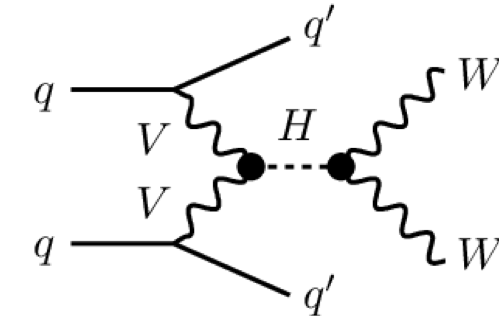
\includegraphics[width=60mm]{./VBF_fainman.png}
    \end{center}
  \end{minipage}
  \begin{minipage}{0.5\hsize}
    \begin{center}
    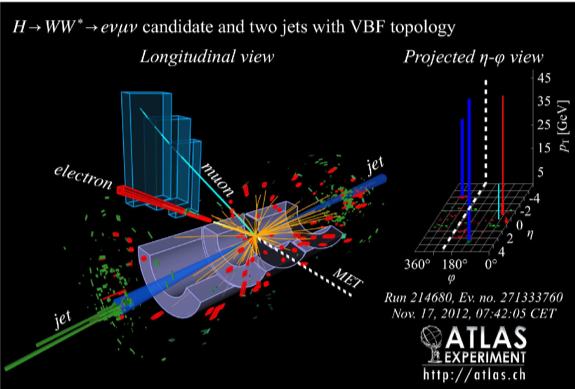
\includegraphics[width=60mm]{./VBF_event_display.png}
    \end{center}
  \end{minipage}
  \caption[VBFイベントの図]{VBFイベントの図\cite{1-8}。図はVBFイベントの一つである$H\rightarrow WW$崩壊チャンネルを示している。左図はファインマン図、右図はそのイベントディスプレイを表す。このイベントにおいて、初めに相互作用したクオーク対は、それぞれ崩壊を繰り返しジェットと呼ばれる粒子群となる。このときこれらのジェットは前方方向に大きな運動量を持つ。ITkでは$|\eta|<4.0$の範囲をカバーしており、このようなジェットを捉えることができるため、測定精度が向上する。}
  \label{VBF_image}
\end{figure}

\begin{table}[bpt]
\begin{center}
\caption[VBF~$H\rightarrow WW$の測定における系統誤差の見積もり]{VBF~$H\rightarrow WW$の測定における系統誤差の見積もり。表は統計数3000~$\rm{fb^{-1}}$において、$|\eta| <2.7$、$|\eta| <4.0$の領域を使用した場合のVBF~$H\rightarrow WW$イベント測定における系統誤差の見積もりを示している。$|\eta| <4.0$の領域を使用することで系統誤差が向上する見積もりであることが分かる。ここでは統計誤差は考慮にいれていない。}
\label{VBF_uncertainty}
  \begin{tabular}{|lll|} \hline
    検出器の使用範囲 & $|\eta| <2.7 $ & $|\eta| < 4.0 $ \\ \hline
    系統誤差 & 22$\%$ & 12$\%$ \\ \hline
  \end{tabular}
\end{center}
\end{table}

